% !Mode:: "TeX:UTF-8"
\title{实验五 MapReduce基础入门 实验报告}
\author{江昱峰 21009200038} 
\documentclass {article}
\usepackage[UTF8]{ctex}
\usepackage{graphicx}
\usepackage{float}
\usepackage{hyperref}
\usepackage{makecell}
\begin{document}
	%\begin{sloppypar}
	\maketitle{}
	\section{背景介绍}
		假如有一个需求,统计图书馆书籍数量。你数1号书架,我数2号书架...... 这就是Map。我们人越多,数书就更快。接下来把所有人的统计数加在一起。这就是Reduce。一个简单的MapReduce过程就被我们实现了。
		
		MapReduce的思想核心是分而治之,适用于大量复杂的任务处理场景(大规模数据处理场景)。Map负责分,即把复杂的任务分解为若干个简单的任务来并行处理。可以进行拆分的前提是这些小任务可以并行计算,彼此间几乎没有依赖关系。Reduce负责合,即对Map阶段的结果进行全局汇总。
	
	\section{实验目的}
		实践并掌握MapReduce基础入门,具体包括以下三部分内容:
		\begin{itemize}
			\item Map端程序编写;
			\item Reduce端程序编写;
			\item Driver端程序编写。
		\end{itemize}
	
	\section{实验知识}	
		操作HDFS文件API概述:Hadoop中关于文件操作类基本上全部是在org.apache.hadoop.fs包中,这些API能够支持的操作包含:打开文件,读写文件,删除文件等。
	
	\section{实验要求}
		完成MapReduce基础入门,具体包括以下三部分任务:
		\begin{itemize}
			\item Map端程序编写;
			\item Reduce端程序编写;
			\item Driver端程序编写。
		\end{itemize}
	
	\section{实验环境}
		本次实验实验环境为青椒课堂平台的Linux(Centos 7.5)操作系统。
	
	\section{实验步骤与结果分析}
		\subsection{Map端程序编写}
			\subsubsection{任务1:Map端程序开发例一}
				本节任务当中,要实现WordCount的Map端程序编写,根据Map端编程步骤进行相关练习,理解Map端业务逻辑。
	
				MapReduce项目创建:
				\begin{enumerate}
					\item 项目名:MRDemo。
					\item 包结构:com.hongya.mrdemo。
					\item Map端程序业务类:WordCountMapper。
					\begin{figure}[H]
						\centering
						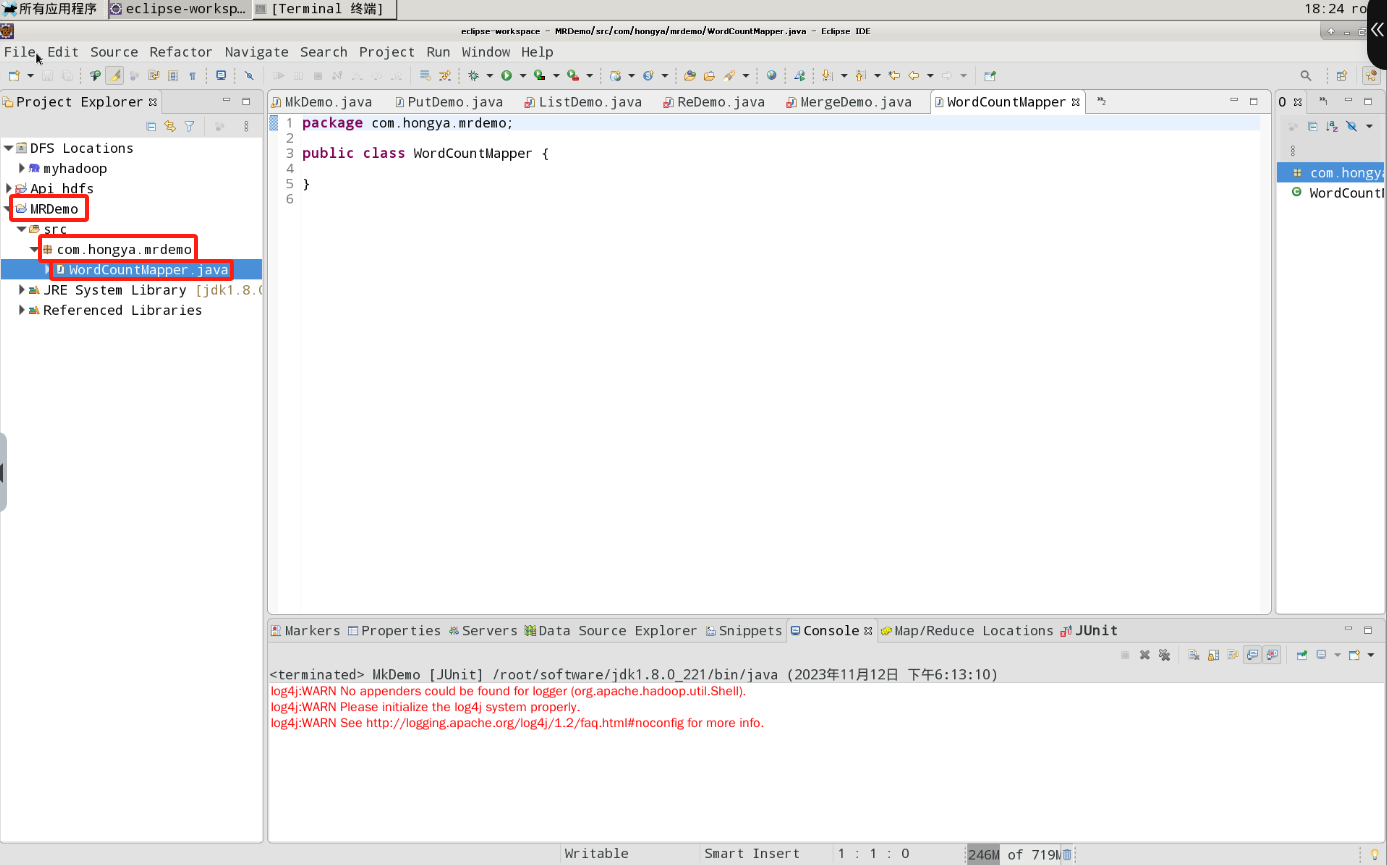
\includegraphics[width=4.5in]{figures/fig1.png}
					\end{figure}
				\end{enumerate}
				
				需求介绍:按照给定的文本,内容如下所示,对其进行WordCount统计,完成Map端程序代码。\\
				hello,hadoop \\
				hello,word \\
				hello,hdfs
				
				Map端编码步骤:
				\begin{enumerate}
					\item 定义的WordCountMapper类继承Mapper,设置泛型类型。
					\item 重写map方法:
					\begin{itemize}
						\item 获取每一行数据并转换成String。
						\item 按逗号切分每行数据获取单词 。
						\item 遍历数组,获取每个单词。
					\end{itemize}
					\item 将单词作为key,value记为1写入上下文。
					\begin{figure}[H]
						\centering
						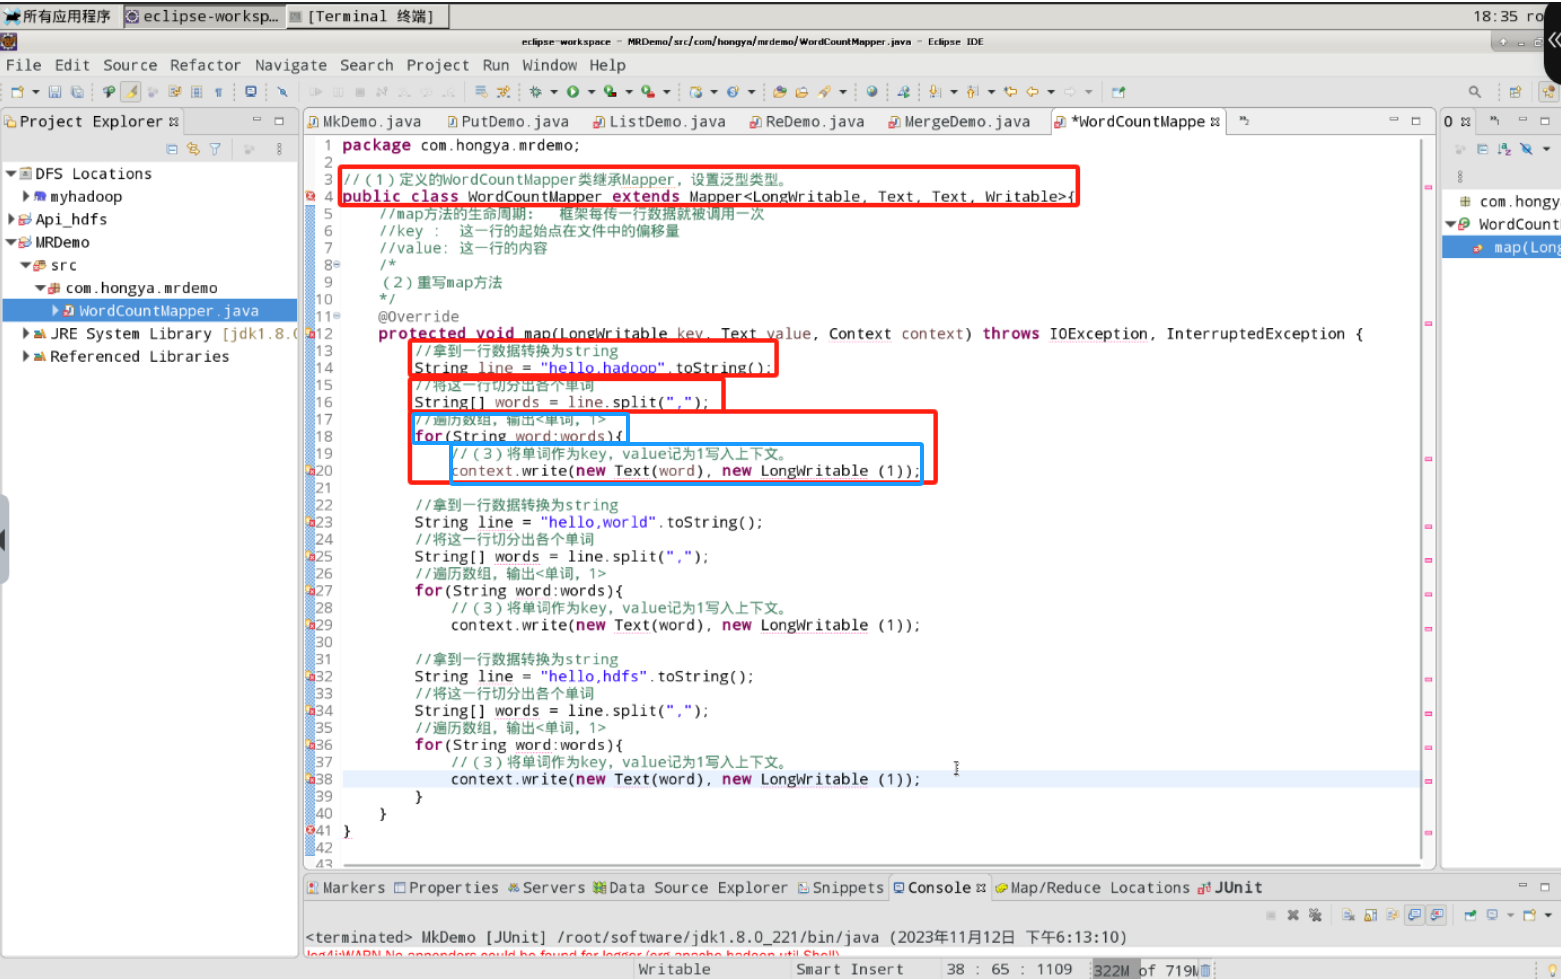
\includegraphics[width=4.5in]{figures/fig2.png}
					\end{figure}
				\end{enumerate}		
			
			\subsubsection{任务2:Map端程序开发例二}	
				准备工作:在任务一包下继续创建类Demo2\_Map进行本节Map端程序开发。	
				
				需求介绍:按照给定的文本,内容如下所示,对其进行WordCount统计,完成Map端程序代码。\\
				hello:world:hadoop \\
				hive:sqoop:lume:hello
				
				Map端编码步骤:
				\begin{enumerate}
					\item 定义的Demo2\_Map类继承Mapper,设置泛型类型。
					\item 重写map方法:
					\begin{itemize}
						\item 获取每一行数据并转换成String。
						\item 切分每行数据获取单词。
						\item 遍历数组,获取每个单词。
					\end{itemize}
					\item 将单词作为key,value记为1写入上下文。
					\begin{figure}[H]
						\centering
						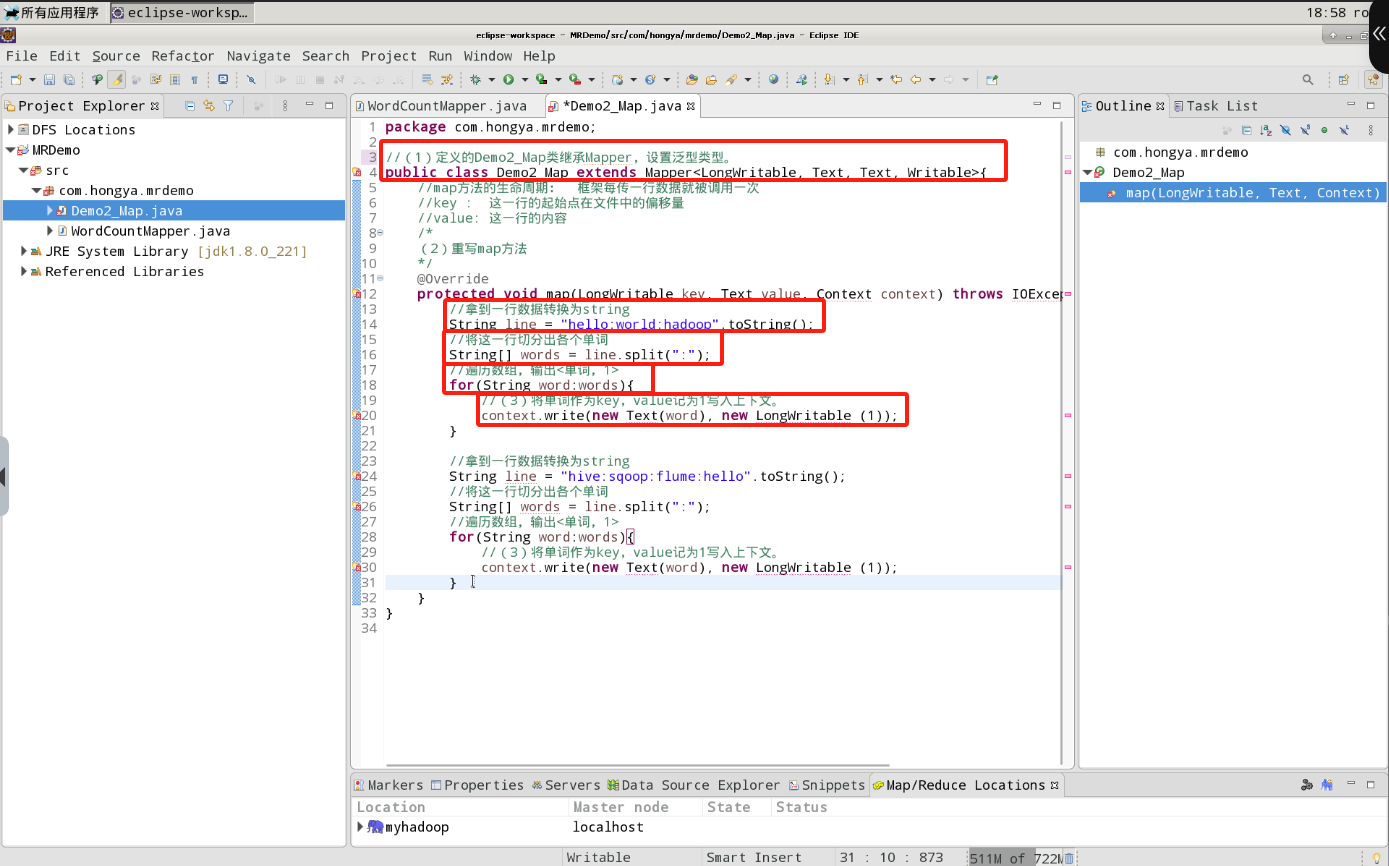
\includegraphics[width=4in]{figures/fig3.png}
					\end{figure}
				\end{enumerate}
			
		\subsection{Reduce端程序编写}
			\subsubsection{Reduce端程序编写例一}
				MapReduce项目创建:
				\begin{enumerate}
					\item 项目名:MRDemo。
					\item 包结构:com.hongya.mrdemo。
					\item Reduce端程序业务类:WordCountReducer。
					\begin{figure}[H]
						\centering
						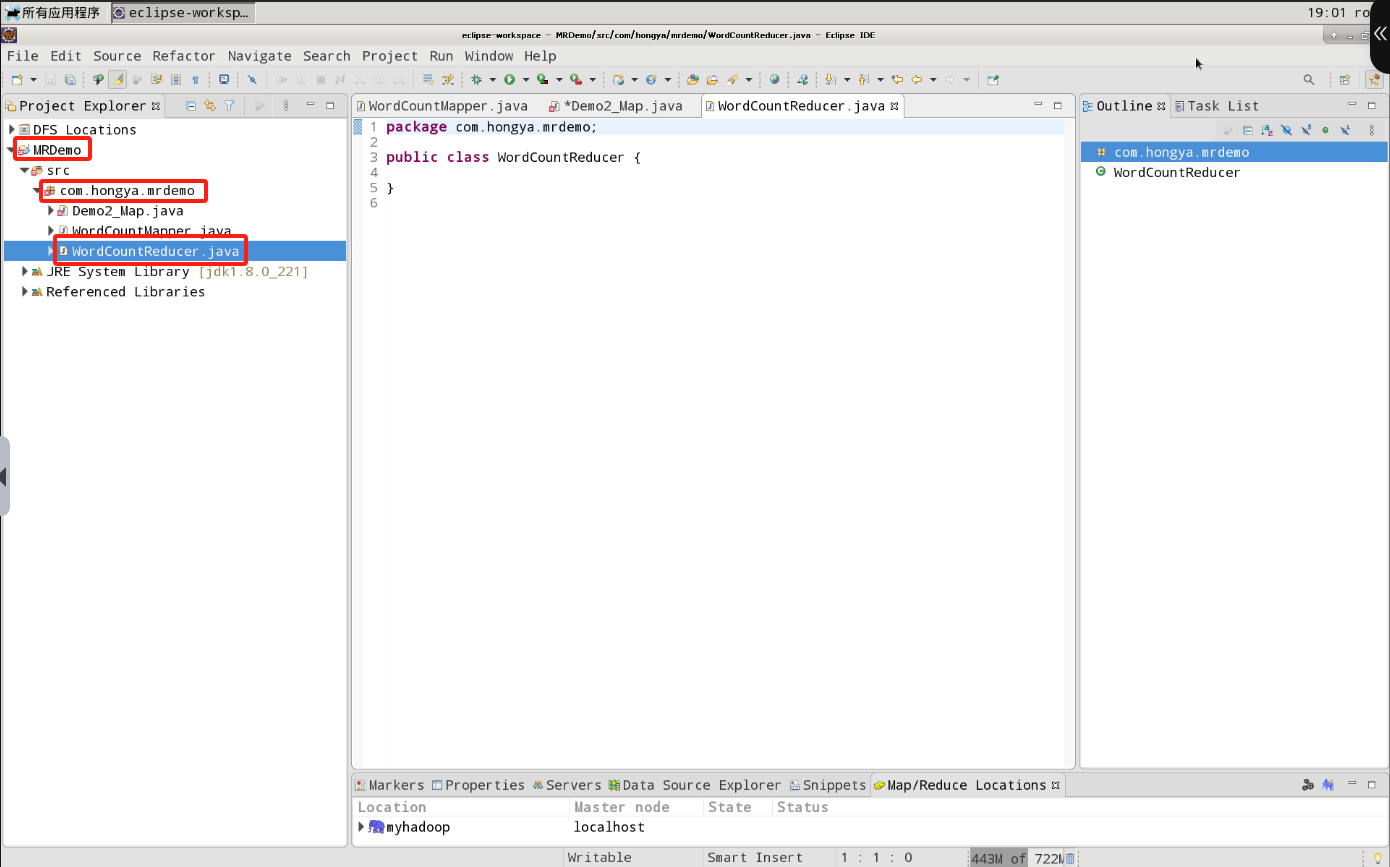
\includegraphics[width=4in]{figures/fig4.png}
					\end{figure}
				\end{enumerate}
			
				Reduce端编程步骤:
				\begin{enumerate}
					\item 定义的WordCountReducer类继承Reducer,设置泛型类型。
					\item 重写reduce方法,对每个单词数求和统计。
					\item 收集统计结果kv写入上下文。
					\begin{figure}[H]
						\centering
						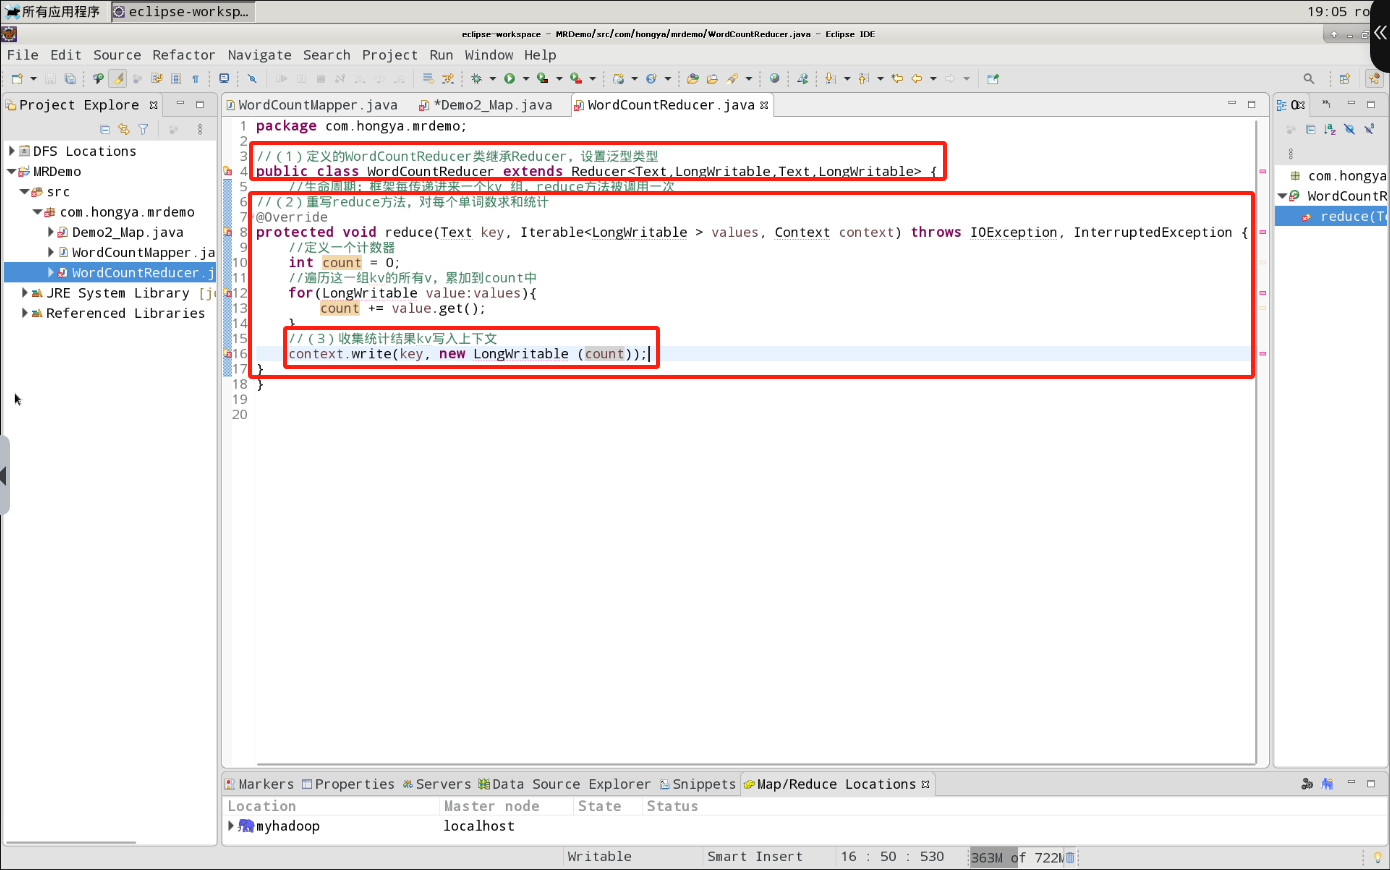
\includegraphics[width=4.5in]{figures/fig5.png}
					\end{figure}
				\end{enumerate}
			
			\subsubsection{任务2:Reduce端程序编写例二}
				准备工作:在任务一包下继续创建类Demo2\_Reduce进行本节Reduce端程序开发。
				
				Reduce端编码步骤:
				\begin{enumerate}
					\item 定义的Demo2\_Reduce类继承Reducer,设置泛型类型。
					\item 重写reduce方法,对每个单词数求和统计。
					\begin{itemize}
						\item 定义计数器count。
						\item 遍历出value并累加到count中。
					\end{itemize}
					\item 收集统计结果kv写入上下文。
					\begin{figure}[H]
						\centering
						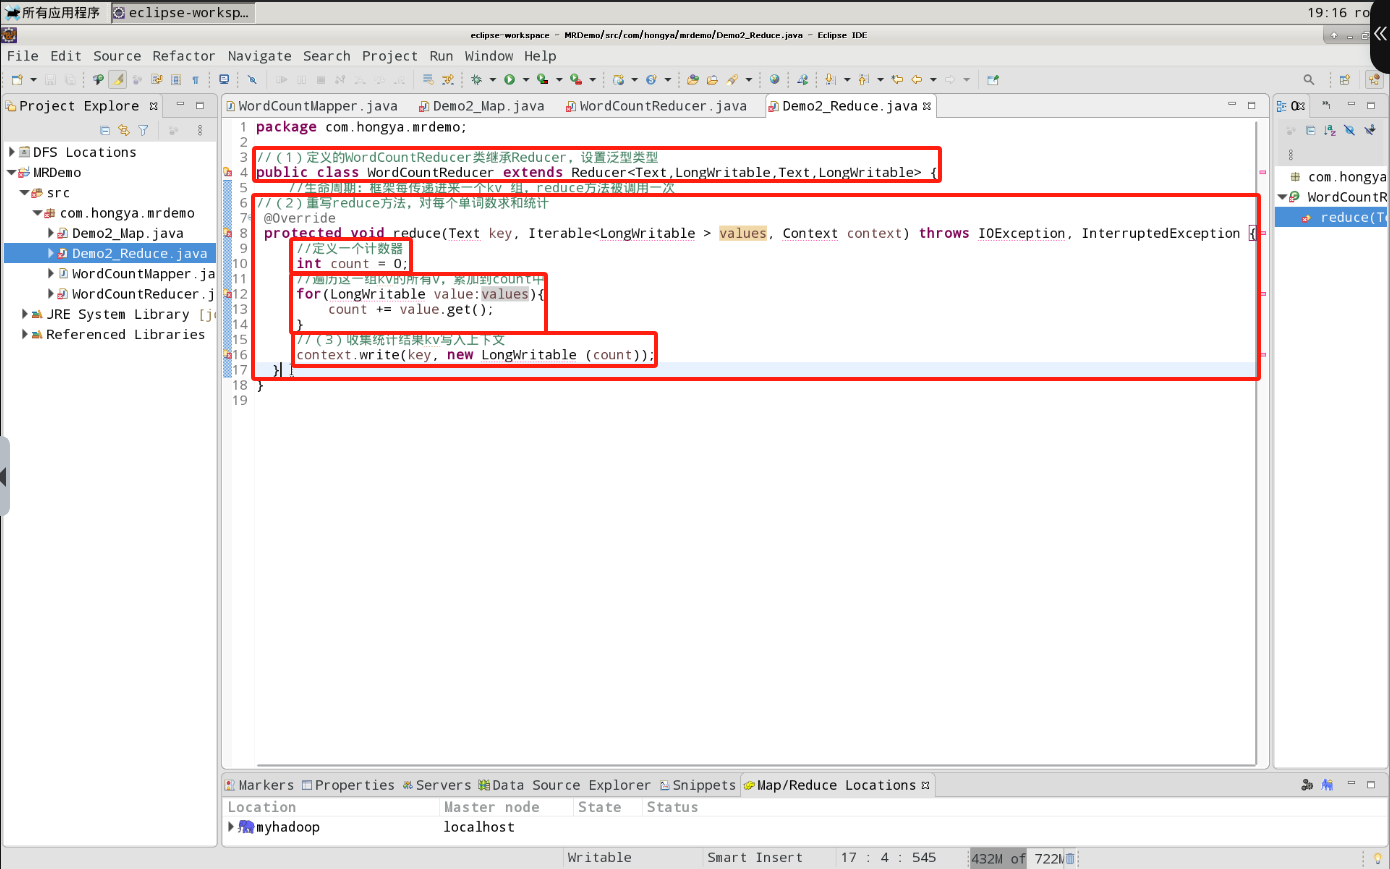
\includegraphics[width=4in]{figures/fig6.png}
					\end{figure}
				\end{enumerate}
			
		\subsection{Driver端程序编写}
			\subsubsection{Driver端程序编写例一}
				MapReduce创建项目:
				\begin{enumerate}
					\item 项目名:MRDemo。
					\item 包结构:com.hongya.mrdemo。
					\item Driver端程序业务类:WordCountDriver。
					\begin{figure}[H]
						\centering
						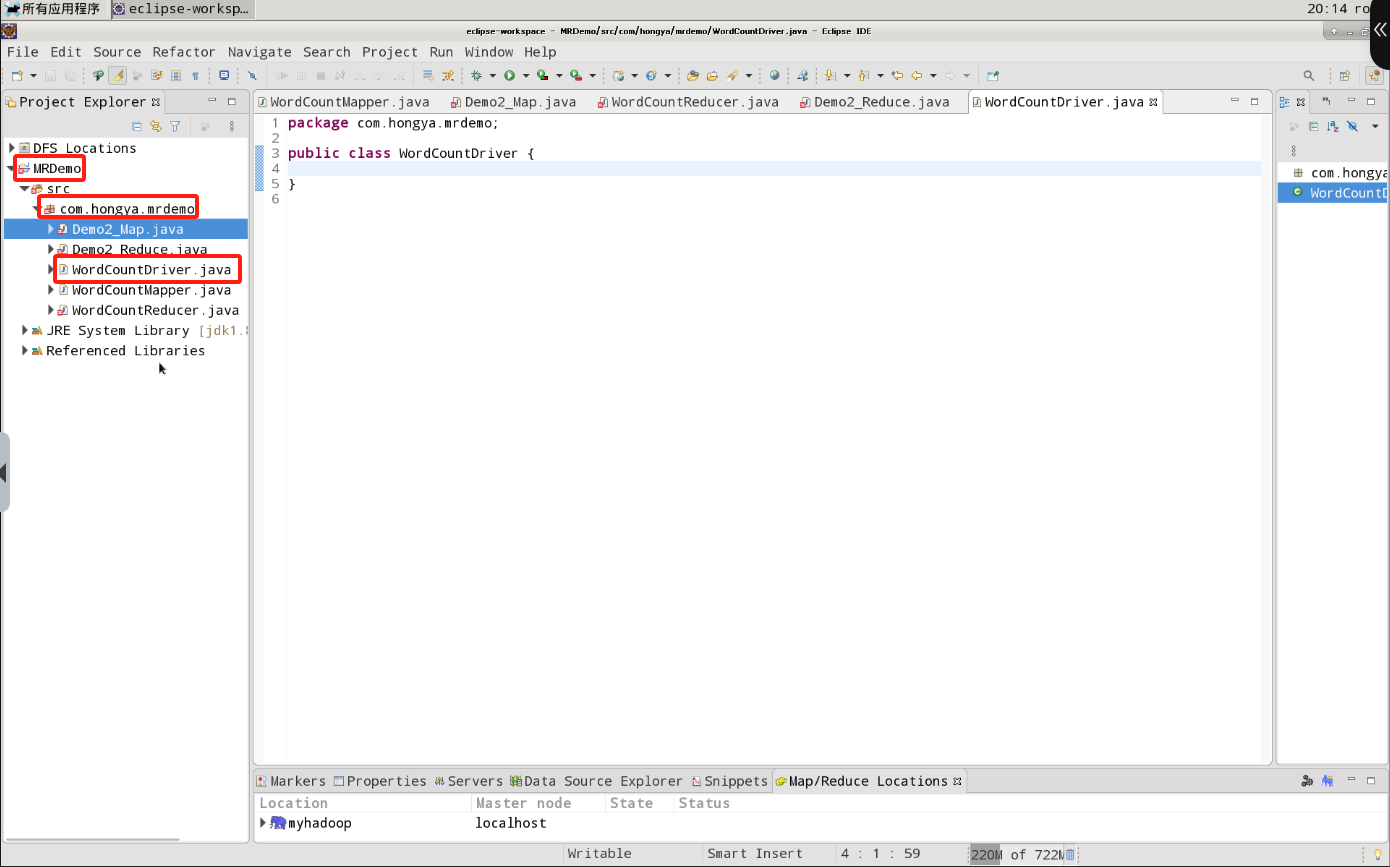
\includegraphics[width=4in]{figures/fig7.png}
					\end{figure}
				\end{enumerate}
			
				准备工作:
				\begin{enumerate}
					\item 点击按钮上传前两节Map和Reduce端代码,上传路径为:/root/eclipse-workspace/MRDemo/src/com/hongya/。
					\begin{figure}[H]
						\centering
						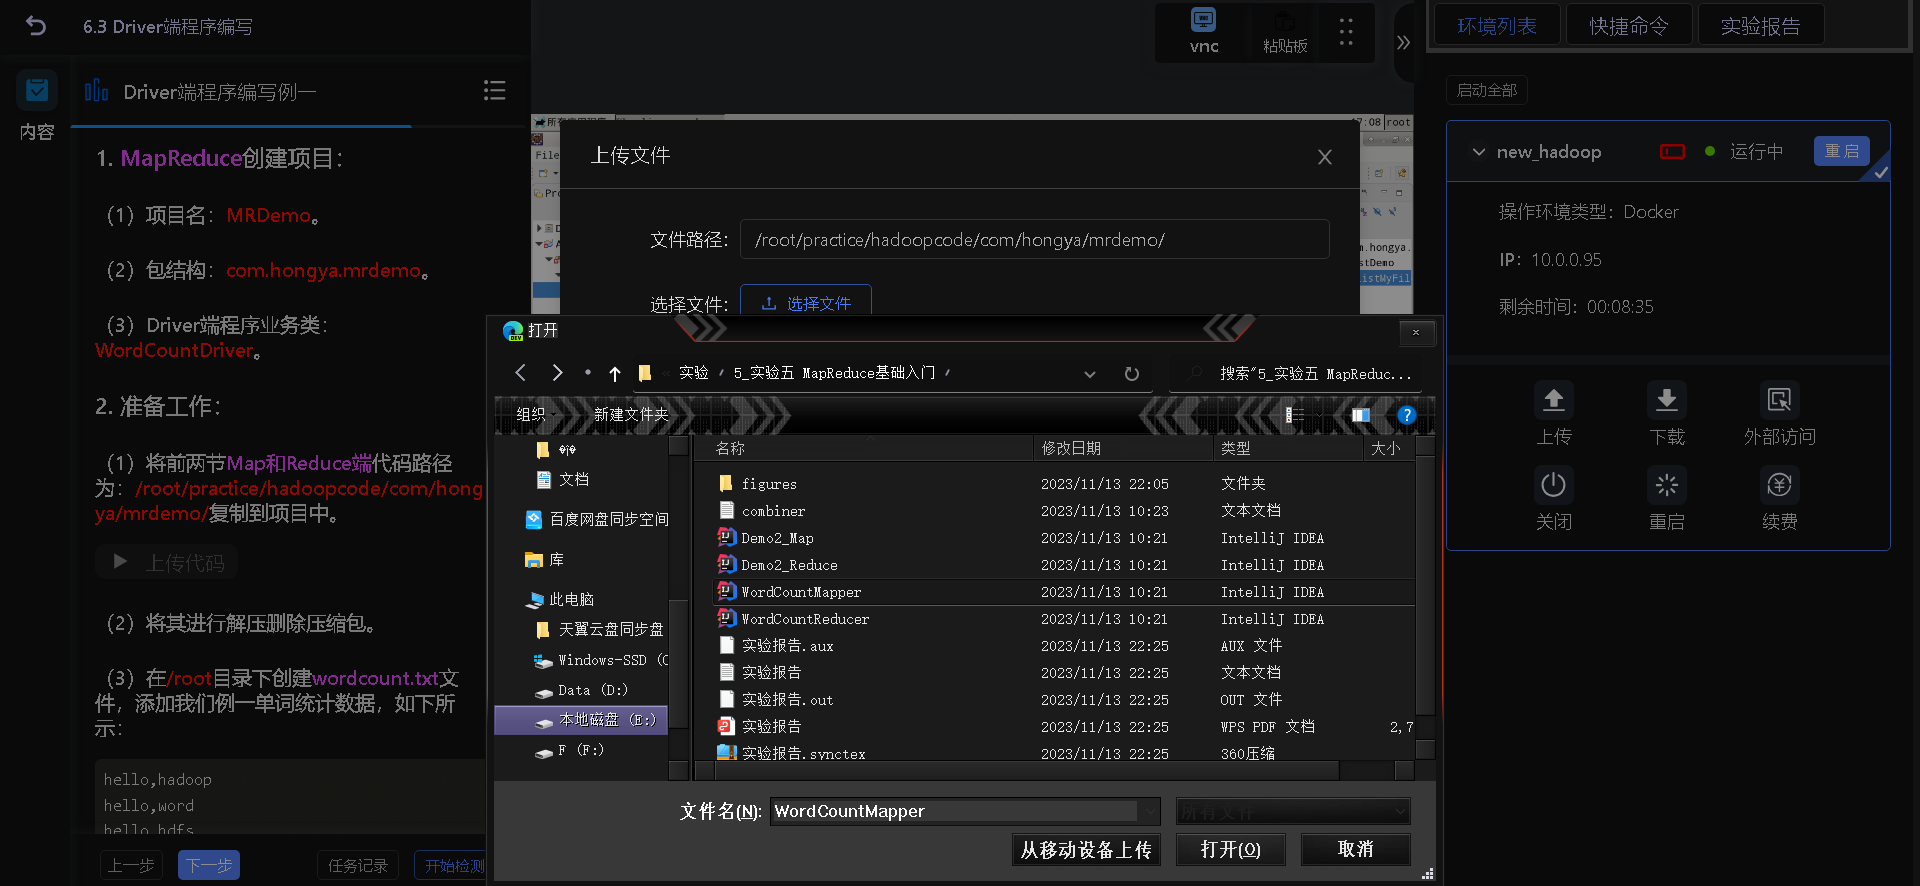
\includegraphics[width=4.5in]{figures/fig7.5.jpg}
					\end{figure}
				
					\item 将其进行解压删除压缩包。
					\item 在/root目录下创建wordcount.txt文件,添加我们例一单词统计数据,如下所示:\\
					hello,hadoop \\
					hello,word \\
					hello,hdfs
					
					\begin{figure}[H]
						\centering
						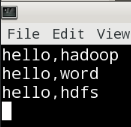
\includegraphics{figures/fig8.png}
					\end{figure}
				\end{enumerate}
			
				Driver端代码逻辑:
				\begin{enumerate}
					\item 在main方法中创建job对象。
					\item 指定job所在的jar包。
					\item 指定Mapper类为例一的WordCountMaaper,Reducer类为例一的WordCountReducer。
					\item 指定MapTask和ReduceTask的输出key-value类型。若两者输出类型一致,MapTask输出类型可省略。
					\item 设置输入路径为/root/wordcount.txt,输出路径为/root/output1。
					\item 将job提交给yarn集群。
					\begin{figure}[H]
						\centering
						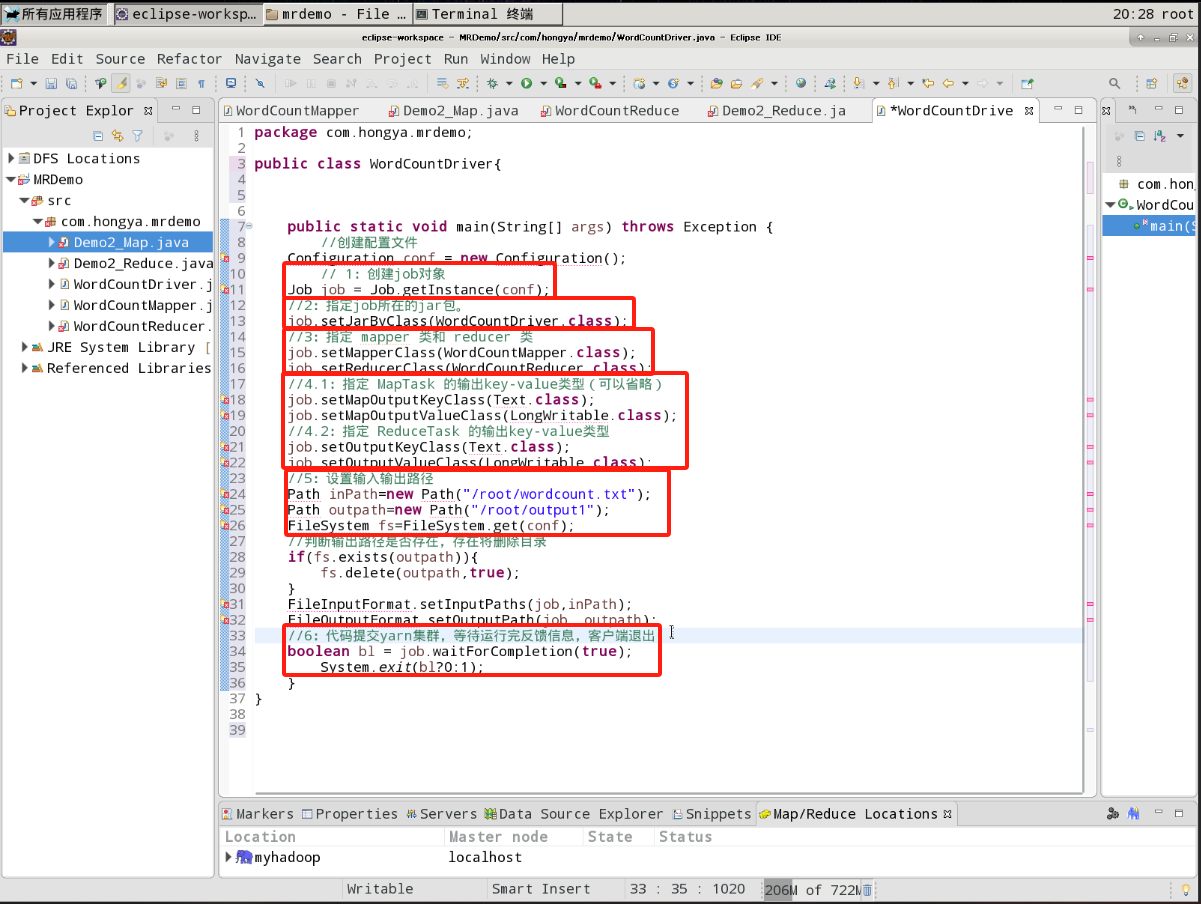
\includegraphics[width=4.5in]{figures/fig9.png}
					\end{figure}
				\end{enumerate}
			
				至此,整个例一单词统计涉及到的程序已经编写完毕,接下来将运行程序查看处理结果。
				
				运行程序并查看结果:
				\begin{enumerate}
					\item 右击WordCountDriver类,选择Run as->Run on Hadoop。
					\begin{figure}[H]
						\centering
						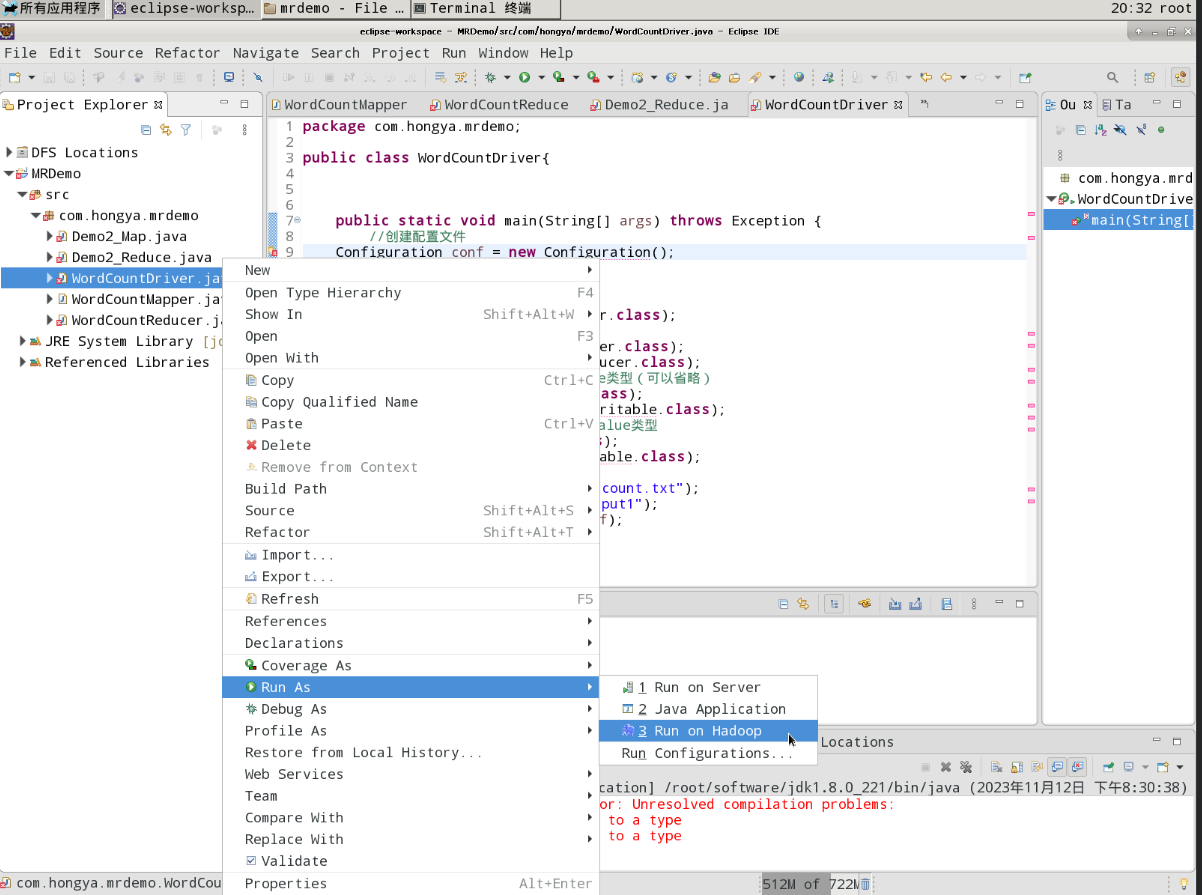
\includegraphics[width=4.5in]{figures/fig10.png}
					\end{figure}
				
					\item 等待程序执行。
					\item 查看输出结果。会在指定的输出路径下生成part-r-00000文件,此文件为输出数据所在文件。
					\begin{figure}[H]
						\centering
						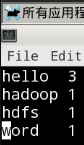
\includegraphics{figures/fig11.png}
					\end{figure}
				\end{enumerate}
			
			\subsubsection{任务2:Driver端程序编写例二}
				准备工作:
				\begin{enumerate}
					\item 在任务一包结构下继续创建例二的Driver端程序类:Demo2\_Driver。
					\item 在/root目录下创建wordcount2.txt文件,添加我们例一单词统计数据,如下所示:\\
					hello:word:hadoop \\
					hive:sqoop:flume:hello
					
					\begin{figure}[H]
						\centering
						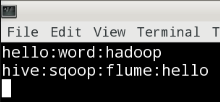
\includegraphics{figures/fig12.png}
					\end{figure}
				\end{enumerate}
			
				Driver端代码逻辑:
				\begin{enumerate}
					\item 在main方法中创建job对象。
					\item 指定job所在的jar包。
					\item 指定Mapper类为例一的Demo2\_Map,Reducer类为例一的Demo2\_Reduce。
					\item 指定MapTask和ReduceTask的输出key-value类型。若两者输出类型一致,MapTask输出类型可省略。
					\item 设置输入路径为/root/wordcount2.txt,输出路径为/root/output2。
					\item 将job提交给yarn集群。
					\begin{figure}[H]
						\centering
						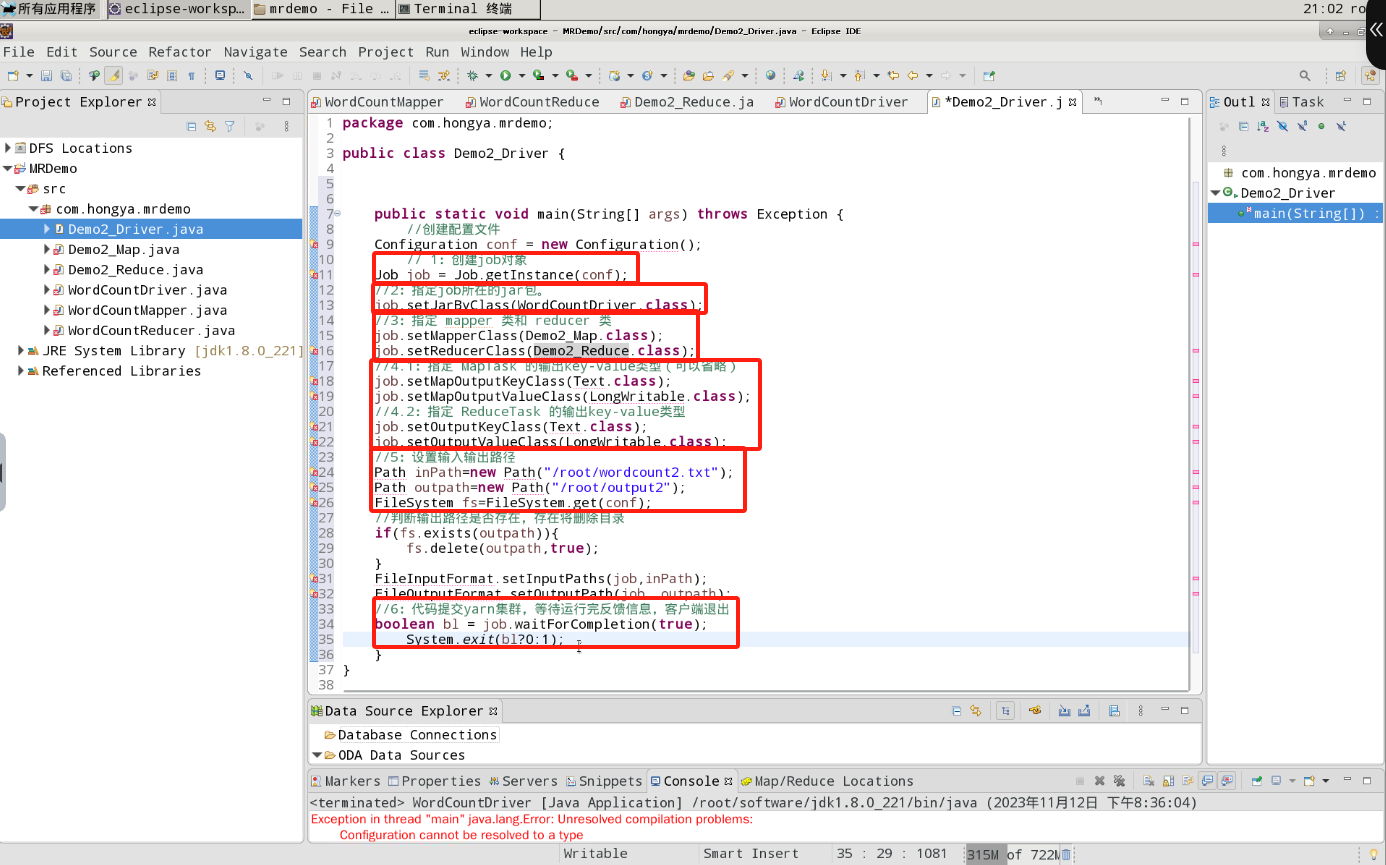
\includegraphics[width=4.5in]{figures/fig13.png}
					\end{figure}
				\end{enumerate}
			
				运行程序并查看结果:
				\begin{enumerate}
					\item 右击WordCountDriver类,选择Run as->Run as Map。
					\begin{figure}[H]
						\centering
						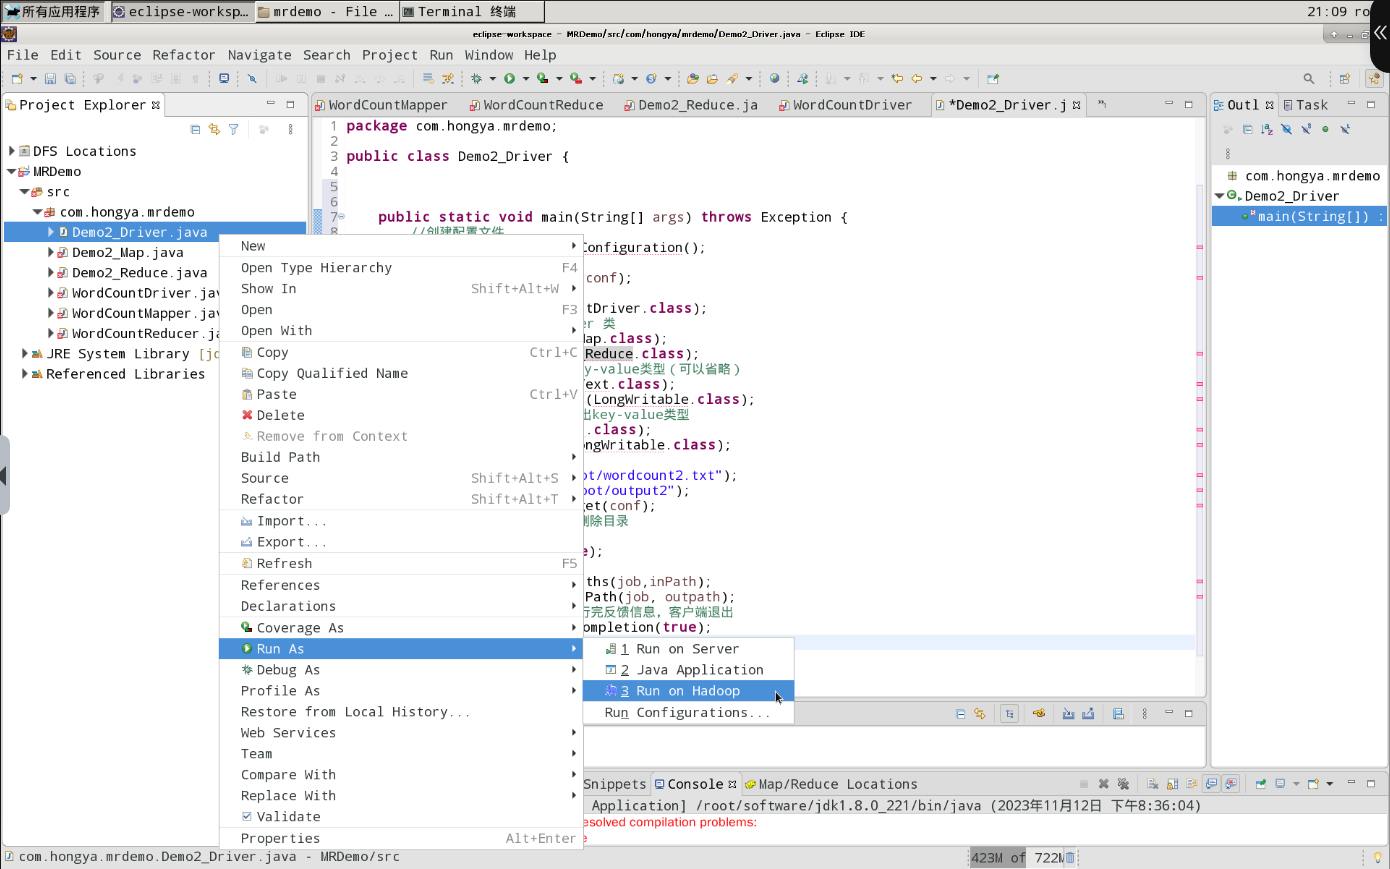
\includegraphics[width=4.5in]{figures/fig14.png}
					\end{figure}
				
					\item 等待程序执行。
					\item 查看输出结果。程序执行成功,会在指定的输出路径下生成part-r-00000文件,此文件为输出数据所在文件。
					\begin{figure}[H]
						\centering
						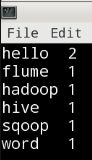
\includegraphics{figures/fig15.png}
					\end{figure}
				\end{enumerate}
			
	\section{结果分析}
		MapReduce整体的作用类似于数据结构中的哈希表,可以分别对不同对象进行计数操作。
	
	\section{困难解决}
		本次实验较为简单,没有遇到困难。
	
	\section{心得体会}
		做完本次实验,除了掌握了实验目的部分中所有内容的收获之外,我还有以下几点心得体会:
		\begin{itemize}
			\item 对比分析了MapReduce和哈希表的异同点;
			\item 掌握了Driver端的功能及其对于Map、Reduce两端的作用。
		\end{itemize}
	
%\end{sloppypar}
\end{document}
\endinput